
\section{A Real-Time Profile for Embedded Java}
\label{sec:rtprof}

As standard Java is under-specified for real-time systems and the
RTSJ does not fit for small embedded systems a new and simpler
real-time profile is defined in this section and implemented on JOP.
The guidelines of the specification are:

\begin{itemize}
\item High-integrity profile
\item Easy syntax
\item Easy to implement
\item Low runtime overhead
\item No syntactic extension of Java
\item Minimum change of Java semantics
\item Support for time measurement if a WCET analysis tool is not available
\item Known overheads (documentation of runtime behavior and memory
requirements of every JVM operation and all methods have to be
provided)
\end{itemize}

The real-time profile under discussion is inspired by the restricted
versions of the RTSJ described in \cite{Pusch01} and
\cite{ravenscar:java}. It is intended for high-integrity real-time
applications and as a test case to evaluate the architecture of JOP
as a Java processor for real-time systems.

The proposed definition is not compatible with the RTSJ. Since the
application domain for the RTSJ is different from high-integrity
systems, it makes sense for it \emph{not} to be compatible with the
RTSJ. Restrictions can be enforced by defining new classes (e.g.\
setting thread priority in the constructor of a real-time thread
alone, enforcing minimum interarrival times for sporadic events).

To verify that this specification is expressive enough for
high-integrity real-time applications, Ravenscar-Java (RJ)
\cite{ravenscar:java}, with the additional necessary RTSJ classes,
has been implemented on top of it. However, RJ inherits some of the
complexity of the RTSJ. Therefore, the implementation of RJ has a
larger memory and runtime overhead than this simple specification.

When the specification for Safety-Critical Java (JSR
302)\footnote{\url{http://jcp.org/en/jsr/detail?id=302}}
\cite{scj:as:proceedings} will be finalized the profile will be
adapted for this specification.

\subsection{Application Structure}

The application is divided in two different phases:
\emph{initialization} and \emph{mission}. All non time-critical
initialization, global object allocations, thread creation and
startup are performed in the initialization phase. All classes need
to be loaded and initialized in this phase. The mission phase starts
after invocation of \code{startMission()}. The number of threads is
fixed and the assigned priorities remain unchanged. The following
restrictions apply to the application:

\begin{itemize}
\item Initialization and mission phase
\item Fixed number of threads
\item Threads are created at initialization phase
\item All shared objects are allocated at initialization
\end{itemize}

\subsection{Threads}

Concurrency is expressed with two types of \emph{schedulable
objects}:
\begin{description}
    \item[Periodic activities] are represented by threads that execute
in an infinite loop invoking \code{waitForNextPeriod()} to get
rescheduled in predefined time intervals.

    \item[Asynchronous sporadic activities] are represented by event
handlers. Each event handler is in fact a thread, which is released
by an hardware interrupt or a software generated event (invocation
of \code{fire()}). Minimum interarrival time has to be specified on
creation of the event handler.

\end{description}
%
The classes that implement the \emph{schedulable objects} are:
%
\begin{description}
    \item[RtThread] represents a periodic task. As usual task
work is coded in \code{run()}, which gets invoked on
\code{missionStart()}. A scoped memory object can be attached to an
\code{RtThread} at creation.

    \item[SwEvent] represents a software-generated event. It is
        triggered by \code{fire()} and needs to override
        \code{handle()}.

\end{description}
%


\begin{lstlisting}[float,caption={Schedulable objects},
label=lst:arch:rt:profile:schobj,{emph=RtThread,enterMemory,
exitMemory,run,waitForNextPeriod,startMission,HwEvent,handle,
SwEvent,fire,handle}]

public class RtThread {

    public RtThread(int priority, int period)
    public RtThread(int priority, int period, int offset)
    public RtThread(int priority, int period, Memory mem)
    public RtThread(int priority, int period, int offset,
                    Memory mem)

    public void setProcessor(int id)

    public void run()
    public boolean waitForNextPeriod()

    public static void startMission()

    public static void sleepMs(int millis)
    public static void busyWait(int us)
    public static RtThread currentRtThread()
}

public class SwEvent extends RtThread {

    public SwEvent(int priority, int minTime)
    public SwEvent(int priority, int minTime, Memory mem)

    public final void fire()
    public void handle()
}
\end{lstlisting}

Listing~\ref{lst:arch:rt:profile:schobj} shows the definition of the
basic classes. Listing~\ref{lst:arch:rt:profile:example} shows the
principle coding of a worker thread. An example for creation of two
real-time threads and an event handler can be seen in
Listing~\ref{lst:arch:rt:profile:usage}.

\begin{lstlisting}[float,caption={A periodic real-time thread},
label=lst:arch:rt:profile:example]

public class Worker extends RtThread {

    private SwEvent event;

    public Worker(int p, int t,
                    SwEvent ev) {

        super(p, t,
            // create a scoped memory area
            new Memory(10000)
        );
        event = ev;
        init();
    }

    private void init() {
        // all initialzation stuff
        // has to be placed here
    }

    public void run() {

        for (;;) {
            work();       // do some work
            event.fire(); // and fire an event

            // wait for next period
            if (!waitForNextPeriod()) {
                missedDeadline();
            }
        }
        // should never reach this point
    }
}
\end{lstlisting}

\begin{lstlisting}[float=t,caption={Start of the application},
label=lst:arch:rt:profile:usage]
    // create an Event
    Handler h = new Handler(3, 1000);

    // create two worker threads with
    // priorities according to their periods
    FastWorker fw = new FastWorker(2, 2000);
    Worker w = new Worker(1, 10000, h);

    // change to mission phase for all
    // periodic threads and event handler
    RtThread.startMission();

    // do some non real-time work
    // and invoke sleep() or yield()
    for (;;) {
        watchdogBlink();
        RtThread.sleepMs(500);
    }
\end{lstlisting}



\subsection{Scheduling}

The scheduler is a preemptive, priority-based scheduler with
unlimited priority levels and a unique priority value for each
schedulable object. No real-time threads or events are scheduled
during the initialization phase.

The design decision to use unique priority levels, instead of FIFO
within priorities, is based on following facts: Two common ways to
assign priorities are rate monotonic and, in a more general form,
deadline monotonic assignment. When two tasks are given the same
priority, we can choose one of them and assign a higher priority to
that task and the task set will still be schedulable. This results
in a strictly monotonic priority order and we do not need to deal
with FIFO order. This eliminates queues for each priority level and
results in a single, priority ordered task list with unlimited
priority levels.

Synchronized blocks are executed with priority ceiling emulation
protocol. In the current implementation top priority is assumed for
all objects. This avoids priority inversions on objects that are not
accessible from the application (e.g. objects inside a library).


\subsection{Memory}

The profile does not support a garbage collector.\footnote{This
restriction can be relaxed when the real-time GC for JOP is used (see
Chapter~\ref{chap:rtgc}).} All memory should be allocated at the
initialization phase. Without a garbage collector, the heap
implicitly becomes immortal memory (as defined by the RTSJ).
% not yet completely implemented -- just as prototype
%For objects created during the mission phase, a scoped memory is
%provided.\footnote{As we now consider real-time GC as the better
%solution, scopes are not supported in the current implementation of
%the profile.} Each scoped memory area is assigned to one
%\code{RtThread}.
%A scoped memory area cannot be shared between threads. No references
%are allowed from the heap to scoped memory. Scoped memory is
%explicitly entered and left using invocations from the application
%logic. Memory areas are cleared both on creation and when leaving the
%scope (invocation of \code{exitMemory()}), leading to a memory area
%with constant allocation time, as opposed to memory with linear
%allocation time (as the memory type \code{LTMemory} in the RTSJ)
%\cite{Corsaro:2003:DPR}.
Scoped memory is currently in a prototyping stage, but will be
supported in the future.


\subsection{Restrictions on Java}

A list of some of the language features that should be avoided for
WCET analyzable real-time threads and bound memory usage:

\begin{description}
    \item[WCET:] Only analyzable language constructs are allowed
        (see \cite{pusch:maxt:jnl}).

    \item[Static class initialization:] Static class initializer
        are invoked at JVM boot. No cyclic dependency is allowed
        and the initialization order is determined at class link
        time. This violation of the JVM specification is
        necessary for tight WCET values of bytecodes \code{new},
        \code{getstatic}, and \code{putstatic}, which usually
        trigger class initialization.

    \item[Inheritance:] Reduce usage of interfaces and overridden methods.

    \item[String concatenation:] In the immortal memory scope,
        only string concatenation with string literals is
        allowed.

    \item[Finalization:] \code{finalize()} has a weak definition
        in Java. Because real-time systems run \emph{forever},
        objects in the heap, which is immortal in this
        specification, will never be finalized.

    \item[Dynamic Class Loading:] Due to the implementation and WCET analysis
complexity dynamic class loading is avoided.

\end{description}


\subsection{Interaction of RtThread, the Scheduler, and the JVM}


\figurename~\ref{fig_arch_rt_user_interaction} shows an interaction
example of the scheduler, the application, and the JVM. The
interaction diagram shows the message sequences between two
application tasks, the scheduler, the JVM and the hardware. The
hardware represents interrupt and timer logic. Task 2 is a periodic
task with a higher priority than Task 1.

\begin{figure*}
    \centering
    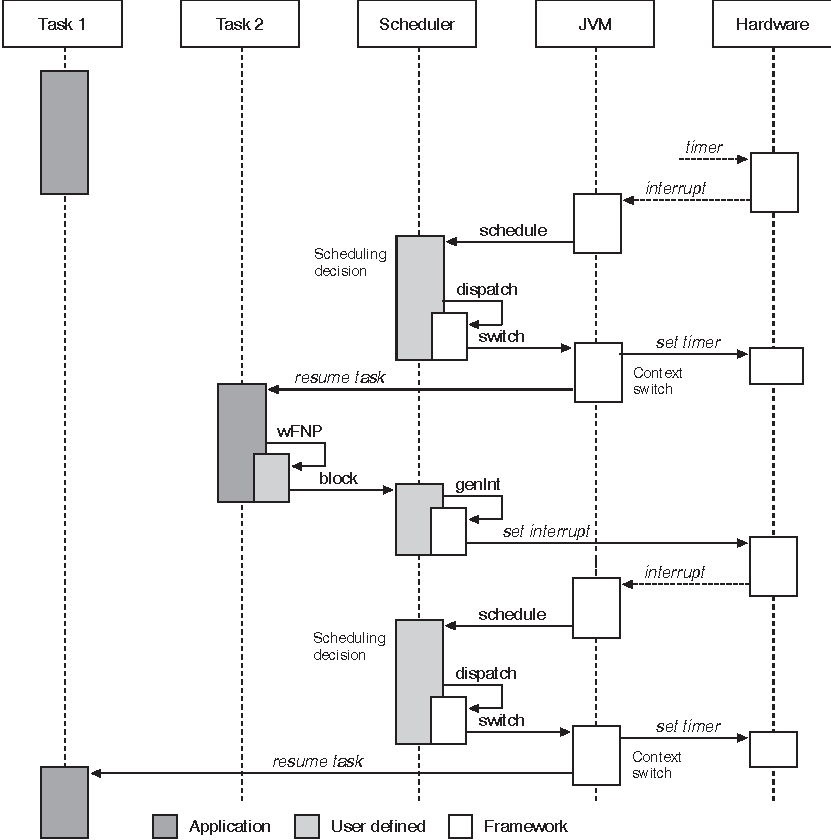
\includegraphics[scale=\picscale]{runtime/rt_user_interaction}
    \caption[Interaction diagram of the scheduler framework]
    {Interaction and message exchange between the application,
the scheduler, the JVM, and the hardware}
    \label{fig_arch_rt_user_interaction}
\end{figure*}

The first event is a timer event to unblock Task 2 for a new period.
The generated timer event results in a call of the scheduler. The
scheduler performs its scheduling decision and issues a context
switch to Task 2. With every context switch the timer is reprogrammed
to generate an interrupt at the next time triggered event for a
higher priority task. Task 2 performs the periodic work and ceases
execution by invocation of \code{waitForNextPeriod()}. The scheduler
is called and requests an interrupt from the hardware resulting in
the same call sequence as with a timer. The software generated
interrupt imposes negligible overhead and results in a single entry
point for the scheduler. Task 1 is the only ready task in this
example and is resumed by the scheduler.

\subsection{Implementation Results}

The initial idea was to implement scheduling and dispatching in
microcode. However, many Java bytecodes have a one to one mapping to
a microcode instruction, resulting in a single cycle execution. The
performance gain of an algorithm coded in microcode is therefore
negligible. As a result, almost all of the scheduling is implemented
in Java. Only a small part of the dispatcher, a memory copy, is
implemented in microcode and exposed with a special bytecode.

Experimental results of basic scheduling benchmarks, such as periodic
thread jitter, context switch time for threads and asynchronous
events, can be found in \cite{jop:rtjava}.

To implement system functions, such as scheduling, in Java, access to
JVM and processor internal data structures have to be available.
However, Java does not allow memory access or access to hardware
devices. In JOP, this access is provided by additional bytecodes. In
the Java environment, these bytecodes are represented as static
native methods. The compiled invoke instruction for these methods
(\code{invokestatic}) is replaced by these additional bytecodes in
the class file. This solution provides a very efficient way to
incorporate low-level functions into a pure Java system. The
translation can be performed during class loading to avoid
non-standard class files.

A pure Java system, without an underlying RTOS, is an unusual system
with some interesting new properties. Java is a safer execution
environment than C (e.g.\ no pointers) and the boundary between
\emph{kernel} and \emph{user space} can become quite loose.
Scheduling, usually part of the operating system or the JVM, is
implemented in Java and executed in the same context as the
application.

This property provides an easy path to a framework for user-defined
scheduling. In \cite{jop:javasched} a framework for a user defined
scheduler for JOP is presented. The events that result in the
scheduling decision are listed. Hooks for these events allow the
implementation of a user defined scheduler.

\subsection{Summary}

This section consider a simple profile for real-time Java and the
implementation of real-time scheduling on a Java processor. The
novelty of the described approach is in implementing functions
usually associated with an RTOS in Java. That means that real-time
Java is not based on an RTOS, and therefore not restricted to the
functionality provided by the RTOS. With JOP, a self-contained
real-time system in pure Java becomes possible. The implementation of
the specification is successfully used as the basis for a commercial
real-time application in the railway industry.
